\section{Encodering en lossless compressie}
\label{sec:encodering}

Nadat we de waarden van de kerntensor en factormatrices gequantiseerd hebben, encoderen we deze naar bits, voegen we deze samen in \'e\'en lange bitstring en comprimeren deze met Deflate om de finale compressie te bekomen. We bespreken in deze sectie enkele keuzes die nog gemaakt moeten worden bij de encodering, na een kort deel over de effici\"entie van de implementatie.

\subsection{Encoderingsmethoden}

Er zijn verschillende manieren om gehele getallen uit $\{0, \dots, 2^b - 1\}$ om te zetten naar een bitstring:
\begin{itemize}

\item \textbf{Standaard:} We schrijven het getal in binair, met de meest significante bit eerst.

\item \textbf{Gray-code \cite{ref:graycode}:} Zoals de standaard-encodering, encoderen Gray-codes waarden uit $\{0, \dots, 2^b - 1\}$ elk naar een code van constante lengte ($b$ bits), maar met de eigenschap dat de encodering van twee opeenvolgende getallen altijd verschilt in juist \'e\'en bit. Dit betekent dat, als de meeste waarden geconcentreerd zijn rond een bepaald punt, dat een groot deel van de bits in de encodering van elke waarde nog gelijk zullen zijn. Dit zou eventueel beter gecomprimeerd kunnen worden.

\item \textbf{Huffman-code \cite{ref:huffman_coding}:} Bij Huffman-encodering worden de verschillende symbolen voorgesteld door codewoorden van variabele lengte, zodat veel voorkomende symbolen ge\"encodeerd worden als korte codewoorden. Dit is erg effici\"ent als men de prefix-boom al kent. In ons geval zullen we echter voor elke quantisatieblok de optimale code berekenen en de bijhorende boom opslaan in een simpel binair formaat (gebaseerd op een post van Stack Overflow \cite{ref:huffman_tree}). In dit formaat neemt de boom $(b + 1)*n + n - 1$ bits in, voor een verzameling van $n$ unieke symbolen, elk initieel voorgesteld door $b$ bits (we zullen de bomen ook nog comprimeren met Deflate om de opslag te minimaliseren). Voor grote quantisatieblokken met veel herhalende symbolen is dit dus niet zo groot meer.

\item \textbf{Adaptief:} Voor kleine blokken kan deze \textit{overhead} veroorzaakt door de opslag van de bomen echter een probleem vormen. Om deze reden ontwikkelden we ook een adaptieve methode: voor elke quantisatieblok wordt gekozen uit een Gray-code, benaderende Huffman-code (zie verder) of exacte Huffman-code, op basis van het kleinste geheugengebruik (inclusief de opslag van de boom). Het opstellen en vergelijken van deze verschillende codes voor elke blok kost echter een significante hoeveelheid tijd (zelfs met een optimalisatie waarbij de exacte Huffman-code niet berekend wordt als men op voorhand al ziet dat de boom te groot gaan zijn).\\

\begin{figure}[H]
\centering
\begin{subfigure}{0.44\textwidth}
  \centering
  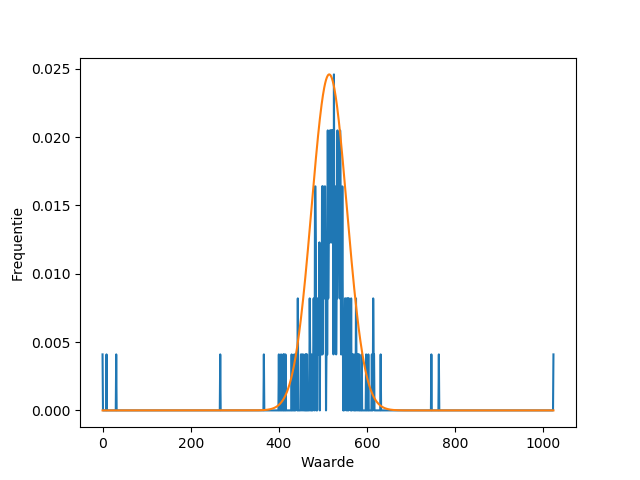
\includegraphics[width=0.9\linewidth]{images/distribution_quantized_values_layer_30.png}
  \caption{Laag 30}
\end{subfigure}
\begin{subfigure}{.44\textwidth}
  \centering
  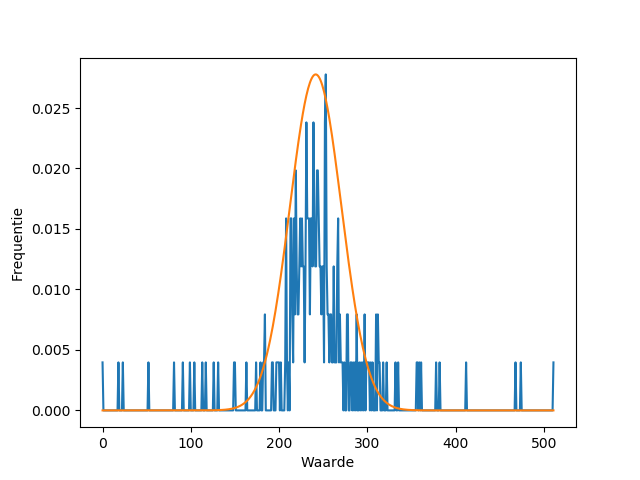
\includegraphics[width=0.9\linewidth]{images/distribution_quantized_values_layer_31.png}
  \caption{Laag 31}
\end{subfigure}
\\
\begin{subfigure}{.44\textwidth}
  \centering
  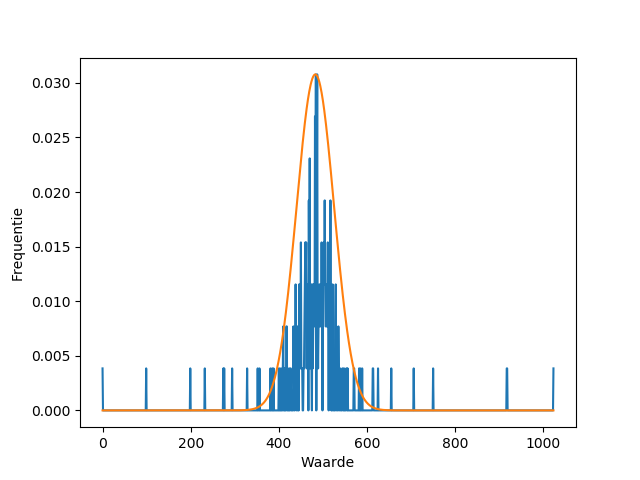
\includegraphics[width=0.9\linewidth]{images/distribution_quantized_values_layer_32.png}
  \caption{Laag 32}
\end{subfigure}
\begin{subfigure}{.44\textwidth}
  \centering
  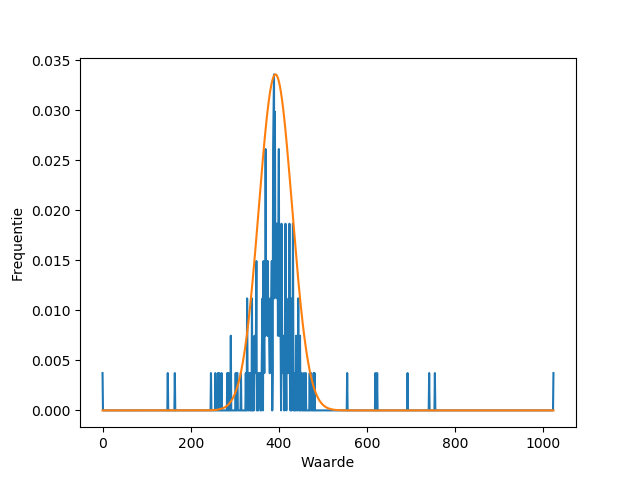
\includegraphics[width=0.9\linewidth]{images/distribution_quantized_values_layer_33.png}
  \caption{Laag 33}
\end{subfigure}
\caption{Verdeling van gequantiseerde waarden binnen een quantisatieblok. Elke grafiek is een voorbeeldblok uit de kerntensor van Cuprite bij relatieve doelfout 0.025. De blauwe lijnen zijn de echte voorkomens (frequenties) van de waarden, de oranje lijnen zijn de Gaussische benaderingen.}
\label{fig:distribution-quantized-values}
\end{figure}

Als men kijkt naar figuur \ref{fig:distribution-quantized-values} ziet men dat voor middelmatig grote quantisatieblokken, er al wat structuur ontstaat in de verdeling van de waarden. Hoewel er nog niet genoeg waarden zijn om een volledige Huffman-boom voor op te slaan, is het gebruik van een standaard encodering of Gray-codes ook niet optimaal.\\

In plaats hiervan introduceren we een nieuwe techniek: een benaderende Huffman-code (BHC). Hierbij berekenen we de Huffman-code, niet met de frequenties van de symbolen in de originele data, maar met de functiewaarden van een Gaussische benadering van deze frequenties. Dit leidt nog steeds tot een redelijk effici\"ente encodering (zie figuur \ref{fig:distribution-quantized-values} voor de nauwkeurigheid van de benadering), want veel voorkomende symbolen zullen door kortere codes voorgesteld worden. De code zelf wordt echter volledig vastgelegd door twee 32-bit floats die de Gaussische benadering defini\"eren ($\mu$ en $\sigma$) en kan dus in slechts 8 bytes opgeslagen worden.\\

In de praktijk betekent dit wel dat men een compleet deterministisch algoritme moet schrijven om de boom te construeren op basis van deze $\mu$ en $\sigma$. Dit zijn echter geen gehele getallen, dus het is niet triviaal om code te schrijven die zelfs na veranderingen in hardware en software nog steeds altijd dezelfde discrete beslissingen neemt op basis van floating-point rekenwerk. Dit lijkt ons mogelijk, maar wel een extra implementatie-uitdaging. In onze onderzoeksomgeving zullen we hier echter geen last van hebben, aangezien we de gecomprimeerde data meteen terug decomprimeren met dezelfde code, dezelfde hardware en dezelfde onderliggende software.

\end{itemize}

\subsection{Endianness}

Uiteindelijk zullen we de bitstring terug moeten omzetten naar een reeks bytes. Elke groep van 8 bits kan dan op twee manieren ge\"interpreteerd worden: met de minst (\textit{little-endian}) of meest (\textit{big-endian}) significante bits eerst. Deze keuze zou technisch gezien een klein effect kunnen hebben op hoe Deflate het resultaat interpreteert en comprimeert, dus we hebben deze beide getest.

\subsection{Implementatie}

We kozen ervoor om de encodering te implementeren met de Python-module \texttt{bitarray} \cite{ref:bitarray}. Aangezien deze in C is geschreven is dit veel sneller dan enige Python-routines dat we zelf zouden kunnen maken. Toch ontbrak er effici\"ente ondersteuning voor twee zaken:

\begin{itemize}

\item De module ondersteunt prefix codes van variabele lengte \cite{ref:variable_length_code} door bij het encoderen/decoderen te vragen naar een \textit{map} van elk symbool naar diens binaire voorstelling. Elke keer wanneer we een quantizatieblok decoderen zal de module echter een boom moeten construeren om snel de bitstring te \textit{parsen}. Deze constructie duurt erg lang en is niet nodig voor codes van constante lengte (zoals de standaard-encodering of Gray-codes). We hebben een nieuwe iterator toegevoegd om te decoderen op basis van zo'n code, waardoor dit proces enorm versneld is.

\item Voor Huffman-codes \cite{ref:huffman_coding} kunnen we deze iterator dus niet gebruiken, want deze codes hebben een variabele lengte. Om dit op te lossen hebben we ook een functie toegevoegd om de prefix-boom door te geven als een bitstring in het formaat dat in de volgende subsectie besproken zal worden. Dit omzeilt de trage omzetting van \textit{map} naar boom en geeft ook een grote versnelling.

\end{itemize}

Verder werd er bij de implementatie van dit deel gebruik gemaakt van van verschillende stukken code van het internet. Aangezien het gaat over algemeen bekende technieken (zoals Gray-codes en Huffman-codes) en geen origineel onderzoek leek dit ons geen probleem. In ieder geval staan alle bronnen van gekopieerde code vermeld in de broncode in bijlage \ref{app:algoritmen}.

\subsection{Besluit}

In tabel \ref{table:encoding-comparison1} vindt men de uiteindelijke groottes van de gecomprimeerde uitvoer. Ten eerste merken we op dat \textit{endianness} geen significant effect heeft, dus we zullen deze vanaf nu altijd als \textit{big-endian} kiezen. Aangezien het comprimeren met Deflate vaak een kleine verbetering geeft, zullen we dit ook standaard doen in de toekomst.\\

\begin{table}[H]
\centering
\begin{tabular}{|l|c|c|c|c|}
\hline
& \multicolumn{2}{c|}{Geen Deflate} & \multicolumn{2}{c|}{Deflate} \\ \cline{1-5} 
\textit{Endianness} & Little & Big & Little & Big \\ \hline
\input{data/encoding-comparison1.tex}                             
\end{tabular}
\caption{Grootte van gecomprimeerde versies van Cuprite (in bytes) voor verschillende encoderingen voor en na compressie met Deflate. Parameters: relatieve doelfout 0.025, bits-parameter voor de kerntensor 12 en bits-parameter voor de factormatrices 10.}
\label{table:encoding-comparison1}
\end{table}

Wanneer we de verschillende encoderingsmethoden bekijken, zien we dat Huffman-encodering eigenlijk veel slechter is dan de standaard encodering of Gray-codes. De verklaring vindt men in tabel \ref{table:encoding-comparison2}: de data zelf wordt significant effici\"enter ge\"encodeerd, maar de bomen kosten te veel ruimte om op te slaan. Hierdoor is de adaptieve encoderingsmethode de beste keuze op vlak van compressiefactor: hierbij worden er alleen Huffman-bomen opgeslagen wanneer dit de totale opslagruimte verlaagt.

\newpage
\begin{table}[H]
\centering
\begin{tabular}{|l|c|c|c|}
\hline
Encoderingsmethode & Ge\"encodeerde data & Bomen & Totaal \\ \hline
\input{data/encoding-comparison2.tex}                             
\end{tabular}
\caption{Grootte van gecomprimeerde versies van Cuprite (in bytes).}
\label{table:encoding-comparison2}
\end{table}

In tabel \ref{table:encoding-timing} zien we echter dat de adaptieve methode veel trager is dan de alternatieven. Om dit aan te pakken zullen we vanaf nu werken met adaptieve encodering waarbij alleen gekozen wordt tussen Gray-codes en exacte Huffman-codes. Het kost namelijk relatief veel tijd om te werken met benaderende Huffman-codes. Op deze manier kunnen we de rekentijd verlagen met een factor 4 terwijl de compressiefactor verschilt met minder dan 0.5\%.

\begin{table}[H]
\centering
\begin{tabular}{|l|c|c|}
\hline
Encoderingsmethode & Relatieve grootte & Totale tijd (s) \\ \hline
\input{data/encoding-timing.tex}                             
\end{tabular}
\caption{Grootte (relatief ten opzichte van het minimum) van gecomprimeerde versies van Cuprite versus uitvoeringstijd voor verschillende encoderingsmethoden (10 experimenten). De totale tijd is hier gedefinieerd als de compressie- en decompressietijd van de quantisatie- en encoderingsfase.}
\label{table:encoding-timing}
\end{table}